\documentclass[12pt]{article}
\usepackage{amsmath}
\usepackage{graphicx}
\usepackage{hyperref}
\usepackage{listings}
\usepackage{color}
\usepackage{pythonhighlight}

\title{Operating System Course Report - First Half of the Semester}
\author{A class}
\date{\today}

\begin{document}

\maketitle
\newpage

\tableofcontents
\newpage

\section{Introduction}
This report summarizes the topics covered during the first half of the Operating System course. It includes theoretical concepts, practical implementations, and assignments. The course focuses on the fundamentals of operating systems, including system architecture, process management, CPU scheduling, and deadlock handling.

\section{Course Overview}
\subsection{Objectives}
The main objectives of this course are:
\begin{itemize}
    \item To understand the basic components and architecture of a computer system.
    \item To learn process management, scheduling, and inter-process communication.
    \item To explore file systems, input/output management, and virtualization.
    \item To study the prevention and handling of deadlocks in operating systems.
\end{itemize}

\subsection{Course Structure}
The course is divided into two halves. This report focuses on the first half, which covers:
\begin{itemize}
    \item Basic Concepts and Components of Computer Systems
    \item System Performance and Metrics
    \item System Architecture of Computer Systems
    \item Process Description and Control
    \item Scheduling Algorithms
    \item Process Creation and Termination
    \item Introduction to Threads
    \item File Systems
    \item Input and Output Management
    \item Deadlock Introduction and Prevention
    \item User Interface Management
    \item Virtualization in Operating Systems
\end{itemize}

\section{Topics Covered}

\subsection{Basic Concepts and Components of Computer Systems}
This section explains the fundamental components that make up a computer system, including the CPU, memory, storage, and input/output devices.

\subsection{System Performance and Metrics}
This section introduces various system performance metrics used to measure the efficiency of a computer system, including throughput, response time, and utilization.

\subsection{System Architecture of Computer Systems}
Describes the architecture of modern computer systems, focusing on the interaction between hardware and the operating system.

\subsection{Process Description and Control}
Processes are a central concept in operating systems. This section covers:
    \subsubsection{Process Description}
    Sebuah proses adalah sebuah program yang sedang dijalankan pada komputer. Setiap proses membutuhkan sumber daya, seperti CPU, memori, dan perangkat \textit{input/output}, untuk bisa berfungsi dengan baik. Komputer harus mengelola berbagai proses agar semua program dapat berfungsi dengan baik. Dalam pengelolaan ini, setiap proses memiliki \textit{process state} dan \textit{process control block} (PCB) yang membantu sistem untuk mengawasi dan mengatur kondisi serta informasi penting mengenai proses tersebut.
    \subsubsection{Process States and State Transitions}
\begin{figure}[h]
    \centering
    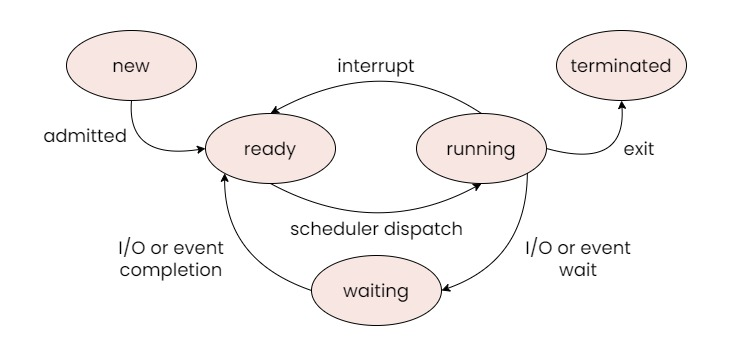
\includegraphics[width=0.8\textwidth]{asset/process-state.jpg}
    \caption{Process states and state transitions}
    \label{fig:process_state}
\end{figure}

\noindent Siklus hidup proses dalam sistem operasi terdiri dari beberapa status, seperti yang terlihat pada gambar di atas. Status-status tersebut meliputi:
\begin{itemize}
    \item \textbf{\textit{New}}: Proses baru saja dibuat dan sedang menunggu  untuk dimasukkan dalam daftar proses yang siap dijalankan. Proses akan berada dalam status ini hingga sistem menerima proses tersebut.
    \item \textbf{\textit{Ready}}: Setelah diterima, proses akan berpindah ke status \textit{ready}. Proses sudah siap untuk dieksekusi namun harus menunggu hingga \textit{scheduler} memilihnya untuk dieksekusi.
    \item \textbf{\textit{Running}}: Proses sedang dieksekusi oleh CPU. Setelah dijadwalkan, proses akan berpindah dari status \textit{ready} ke \textit{running}.
    \item \textbf{\textit{Waiting}}: Proses sedang menunggu operasi I/O atau suatu \textit{event} tertentu. Ketika proses membutuhkan input dari perangkat keras atau menunggu suatu \textit{event}, ia akan berpindah dari status running ke \textit{waiting}.
    \item \textbf{\textit{Terminated}}: Proses telah selesai dieksekusi. Setelah eksekusi selesai, proses akan berpindah dari status \textit{running} ke \textit{terminated}, di mana ia tidak lagi menjadi bagian dari sistem.
\end{itemize}
Transisi antar status tersebut meliputi:
\begin{itemize}
    \item \textbf{\textit{Admitted}}: Ketika sebuah proses baru dibuat, ia akan berpindah dari status \textit{new} ke \textit{ready} setelah diterima oleh sistem operasi.
    \item \textbf{\textit{Scheduler Dispatch}}: Ketika CPU siap untuk mengeksekusi proses, penjadwal akan memindahkan proses dari status \textit{ready} ke \textit{running}.
    \item \textbf{\textit{I/O or Event Wait}}: Ketika proses membutuhkan operasi I/O atau menunggu suatu kejadian, proses akan berpindah dari \textit{running} ke \textit{waiting}.
    \item \textbf{\textit{I/O or Event Completion}}: Setelah operasi I/O atau kejadian selesai, proses yang berada di status \textit{waiting} akan berpindah kembali ke status \textit{ready}.
    \item \textbf{\textit{Interrupt}}: Jika proses yang sedang berjalan terganggu (misalnya oleh penjadwal untuk memberikan giliran kepada proses lain), proses akan berpindah dari \textit{running} ke \textit{ready}.
    \item \textbf{\textit{Exit}}: Ketika proses selesai dieksekusi, ia akan berpindah dari \textit{running} ke \textit{terminated}.
\end{itemize}
    \subsubsection {Process Control Block (PCB)}
    \subsubsection {Process Control}
    \begin{thebibliography}{9}
    \bibitem{Silberschatz2009} 
    Silberschatz, A., Galvin, P. B., \& Gagne, G. (2009). \textit{Operating System Concepts} (8th ed.). Hoboken, NJ: Wiley.
    \end{thebibliography}

\subsection{Scheduling Algorithms}
This section covers:
\begin{itemize}
    \item First-Come, First-Served (FCFS)
    \item Shortest Job Next (SJN)
    \item Round Robin (RR)
\end{itemize}
It explains how these algorithms are used to allocate CPU time to processes.

\subsection{Process Creation and Termination}
Details how processes are created and terminated by the operating system, including:
\begin{itemize}
    \item Process spawning
    \item Process termination conditions
\end{itemize}

\subsection{Introduction to Threads}
This section introduces the concept of threads and their relation to processes, covering:
\begin{itemize}
    \item Single-threaded vs. multi-threaded processes
    \item Benefits of multithreading
\end{itemize}

\begin{figure}[h]
    \centering
    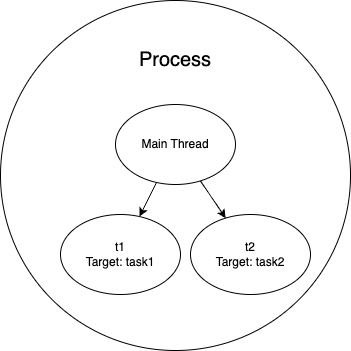
\includegraphics[width=0.5\textwidth]{/Users/khawaritzmi/Unhas/os_report_mid2024/a_class/asset/example.png}  % Sesuaikan nama file dan ukurannya
    \caption{Ini adalah gambar contoh dari multithreading.}
    \label{fig:contoh_gambar}
\end{figure}

Seperti yang terlihat pada Gambar \ref{fig:contoh_gambar}, inilah cara menambahkan gambar dengan keterangan.

\subsection{File Systems}
File systems provide a way for the operating system to store, retrieve, and manage data. This section explains:
\begin{itemize}
    \item File system structure
    \item File access methods
    \item Directory management
\end{itemize}

\subsection{Input and Output Management}
Input and output management is key for handling the interaction between the system and external devices. This section includes:
\begin{itemize}
    \item Device drivers
    \item I/O scheduling
\end{itemize}

\subsection{Deadlock Introduction and Prevention}
Explores the concept of deadlocks and methods for preventing them:
\begin{itemize}
    \item Deadlock conditions
    \item Deadlock prevention techniques
\end{itemize}

\subsection{User Interface Management}
This section discusses the role of the operating system in managing the user interface. Topics covered include:
\begin{itemize}
    \item Graphical User Interface (GUI)
    \item Command-Line Interface (CLI)
    \item Interaction between the user and the operating system
\end{itemize}

\subsection{Virtualization in Operating Systems}
Virtualization allows multiple operating systems to run concurrently on a single physical machine. This section explores:
\begin{itemize}
    \item Concept of virtualization
    \item Hypervisors and their types
    \item Benefits of virtualization in modern computing
\end{itemize}

\section{Assignments and Practical Work}
\subsection{Assignment 1: Process Scheduling}
Students were tasked with implementing various process scheduling algorithms (e.g., FCFS, SJN, and RR) and comparing their performance under different conditions.
\subsubsection{Group 1}
\begin{python}
    class Process:
    def __init__(self, pid, arrival_time, burst_time):
        self.pid = pid
        self.arrival_time = arrival_time
        self.burst_time = burst_time
        self.completion_time = 0
        self.turnaround_time = 0
        self.waiting_time = 0
\end{python}

\begin{table}[htbp] % Optional: For floating position
    \centering
    \begin{tabular}{|c|c|c|} % Defines number of columns and alignment (c = center, l = left, r = right). '|' creates vertical lines.
    \hline
    Header 1 & Header 2 & Header 3 \\ % Column headers
    \hline
    Row 1, Column 1 & Row 1, Column 2 & Row 1, Column 3 \\ % First row of data
    \hline
    Row 2, Column 1 & Row 2, Column 2 & Row 2, Column 3 \\ % Second row of data
    \hline
    \end{tabular}
    \caption{Your table caption} % Optional: For adding a caption
    \label{tab:your_label} % Optional: For cross-referencing the table
\end{table}
\subsection{Assignment 2: Deadlock Handling}
In this assignment, students were asked to simulate different deadlock scenarios and explore various prevention methods.

\subsection{Assignment 3: Multithreading and Amdahl's Law}
This assignment involved designing a multithreading scenario to solve a computationally intensive problem. Students then applied **Amdahl's Law** to calculate the theoretical speedup of the program as the number of threads increased.

\subsection{Assignment 4: Simple Command-Line Interface (CLI) for User Interface Management}
Students were tasked with creating a simple **CLI** for user interface management. The CLI should support basic commands such as file manipulation (creating, listing, and deleting files), process management, and system status reporting.

\subsection{Assignment 5: File System Access}
In this assignment, students implemented file system access routines, including:
\begin{itemize}
    \item File creation and deletion
    \item Reading from and writing to files
    \item Navigating directories and managing file permissions
\end{itemize}

\section{Conclusion}
The first half of the course introduced core operating system concepts, including process management, scheduling, multithreading, and file system access. These topics provided a foundation for more advanced topics to be covered in the second half of the course.

\end{document}